%% This file is cloned from `sample-sigconf.tex',
\documentclass[sigconf]{acmart}
%% \BibTeX command to typeset BibTeX logo in the docs
\AtBeginDocument{%
  \providecommand\BibTeX{{%
    Bib\TeX}}}
\setcopyright{acmlicensed}
\copyrightyear{2024}
\acmYear{2024}
\acmDOI{XXXXXXX.XXXXXXX}
\acmConference[EuroPLoP '24]{29th European Conference on Pattern Languages of Programs}{July 3--7, 2024}{Kloster Irsee, Germany}
\acmISBN{978-1-4503-XXXX-X/18/06}
% ============================================================
% ============================================================
\usepackage{xspace}
\usepackage{graphicx}
\graphicspath{{figures/}}
% ============================================================
%% Uncomment the next few lines to get sf url links:
%\usepackage{url}            
%\makeatletter
%\def\url@leostyle{%
%  \@ifundefined{selectfont}{\def\UrlFont{\sf}}{\def\UrlFont{\small\sffamily}}}
%\makeatother
%\urlstyle{leo} % Now actually use the newly defined style.
%% Choose coloured or b/w links:
%\usepackage[pdftex,colorlinks=true,pdfstartview=FitV,
% linkcolor=black,citecolor=black,urlcolor=black]{hyperref}
%\usepackage{hyperref}
\usepackage{needspace}
\newcommand{\needlines}[1]{\Needspace{#1\baselineskip}}
\usepackage{paralist}
% ============================================================
%:Markup macros for proof-reading
\usepackage{ifthen}
\usepackage[normalem]{ulem} % for \sout
\usepackage{xcolor}
\newcommand{\ra}{$\rightarrow$}
\newboolean{showedits}
\setboolean{showedits}{true} % toggle to show or hide edits
%\setboolean{showedits}{false} % toggle to show or hide edits
\ifthenelse{\boolean{showedits}}
{
	\newcommand{\meh}[1]{\textcolor{red}{\uwave{#1}}} % please rephrase
	\newcommand{\ins}[1]{\textcolor{blue}{\uline{#1}}} % please insert
	\newcommand{\del}[1]{\textcolor{red}{\sout{#1}}} % please delete
	\newcommand{\chg}[2]{\textcolor{red}{\sout{#1}}{\ra}\textcolor{blue}{\uline{#2}}} % please change
	\newcommand{\nbe}[3]{
		{\colorbox{#3}{\bfseries\sffamily\scriptsize\textcolor{white}{#1}}}
		{\textcolor{#3}{\sf\small$\blacktriangleright$\textit{#2}$\blacktriangleleft$}}}
}{
	\newcommand{\meh}[1]{#1} % please rephrase
	\newcommand{\ins}[1]{#1} % please insert
	\newcommand{\del}[1]{} % please delete
	\newcommand{\chg}[2]{#2}
	\newcommand{\nbe}[3]{}
}
%
\newcommand\rA[1]{\nbe{Reviewer A}{#1}{cyan}}
\newcommand\rB[1]{\nbe{Reviewer B}{#1}{olive}}
\newcommand\rC[1]{\nbe{Reviewer C}{#1}{magenta}}
\newcommand\ANS[1]{\nbe{Response}{#1}{teal}}

\newcommand{\THE}{\ins{the}\xspace} % "the" missing
\newcommand{\A}{\ins{a}\xspace} % "a" missing
\newcommand{\s}{\ins{s}\xspace} % "s" missing
\newcommand{\COMMA}{\ins{,}\xspace} % "," missing
\newcommand{\THAT}{\chg{which}{that}\xspace} % use "that", not "which"

% ============================================================
%:Box comments/edits
\usepackage[most]{tcolorbox}
\ifthenelse{\boolean{showedits}}
{
  \newtcolorbox{inserted}{%
       title=Inserted text:,
       colframe=blue,colback=blue!5!white,
       breakable,
       leftrule=0mm, 
       bottomrule=0mm,
       rightrule=0mm,
       toprule=0mm,
       arc=0mm, outer arc=0mm,
       oversize
  }
  \newtcolorbox{deleted}{%
       title=Deleted text:,
       colframe=red,colback=red!5!white,
       breakable,
       leftrule=0mm, 
       bottomrule=0mm,
       rightrule=0mm,
       toprule=0mm,
       arc=0mm, outer arc=0mm,
       oversize
  }
  \newtcolorbox{refactored}{%
       % title=Heavily modifed/refactored text:,
       title=Rewritten text:,
       colframe=blue,colback=red!5!white,
       breakable,
       leftrule=0mm, 
       bottomrule=0mm,
       rightrule=0mm,
       toprule=0mm,
       arc=0mm, outer arc=0mm,
       oversize
  }
}{
  \newenvironment{inserted}{}{}
  %\newenvironment{deleted}{ \begin{comment} }{ \end{comment} }
  \let\deleted\comment
  \newenvironment{refactored}{}{} 
}
% ============================================================
%:Put edit comments in a really ugly standout display
%\usepackage{ifthen}
%\usepackage{amssymb} % Avoid error: Command `\Bbbk' already defined.
\newboolean{showcomments}
\setboolean{showcomments}{true}
%\setboolean{showcomments}{false}
\newcommand{\id}[1]{$-$Id: scgPaper.tex 32478 2010-04-29 09:11:32Z oscar $-$}
\newcommand{\yellowbox}[1]{\fcolorbox{gray}{yellow}{\bfseries\sffamily\scriptsize#1}}
\newcommand{\triangles}[1]{{\sf\small$\blacktriangleright$\textit{#1}$\blacktriangleleft$}}
\ifthenelse{\boolean{showcomments}}
%{\newcommand{\nb}[2]{{\yellowbox{#1}\triangles{#2}}}
{\newcommand{\nbc}[3]{
 {\colorbox{#3}{\bfseries\sffamily\scriptsize\textcolor{white}{#1}}}
 {\textcolor{#3}{\sf\small$\blacktriangleright$\textit{#2}$\blacktriangleleft$}}}
 \newcommand{\version}{\emph{\scriptsize\id}}}
{\newcommand{\nbc}[3]{}
 \newcommand{\version}{}}
\newcommand{\nb}[2]{\nbc{#1}{#2}{orange}}
\newcommand{\here}{\yellowbox{$\Rightarrow$ CONTINUE HERE $\Leftarrow$}}
\newcommand\rev[2]{\nb{TODO (rev #1)}{#2}} % reviewer comments
\newcommand\fix[1]{\nb{FIX}{#1}}
\newcommand\todo[1]{\nb{TO DO}{#1}}
\newcommand\on[1]{\nbc{ON}{#1}{olive}} % add more author macros here
\newcommand\tg[1]{\nbc{TG}{#1}{blue}}
%\newcommand\XXX[1]{\nbc{XXX}{#1}{brown}}
%\newcommand\XXX[1]{\nbc{XXX}{#1}{cyan}}
%\newcommand\XXX[1]{\nbc{XXX}{#1}{darkgray}}
%\newcommand\XXX[1]{\nbc{XXX}{#1}{gray}}
%\newcommand\XXX[1]{\nbc{XXX}{#1}{magenta}}
%\newcommand\XXX[1]{\nbc{XXX}{#1}{olive}}
%\newcommand\XXX[1]{\nbc{XXX}{#1}{orange}}
%\newcommand\XXX[1]{\nbc{XXX}{#1}{purple}}
%\newcommand\XXX[1]{\nbc{XXX}{#1}{red}}
%\newcommand\XXX[1]{\nbc{XXX}{#1}{teal}}
%\newcommand\XXX[1]{\nbc{XXX}{#1}{violet}}
% ============================================================
\newboolean{isblinded}
\setboolean{isblinded}{true}
%\setboolean{isblinded}{false}
\ifthenelse{\boolean{isblinded}}
{\newcommand\blind[1]{BLINDED\xspace}}
{\newcommand\blind[1]{#1\xspace}}
% ============================================================
\newcommand{\seclabel}[1]{\label{sec:#1}}
%\newcommand{\secref}[1]{Section~\ref{sec:#1}} <- use \autoref instead!
\newcommand{\figlabel}[1]{\label{fig:#1}}
%\newcommand{\figref}[1]{Figure~\ref{fig:#1}}
\newcommand{\tablabel}[1]{\label{tab:#1}}
%\newcommand{\tabref}[1]{Table~\ref{tab:#1}}
% ============================================================
\newcommand{\ie}{\emph{i.e.},\xspace}
\newcommand{\eg}{\emph{e.g.},\xspace}
\newcommand{\etal}{\emph{et al.}\xspace}
\newcommand{\etc}{\emph{etc.}\xspace}
% ============================================================

% $Author: oscar $
% $Date: 2009-11-06 14:37:12 +0100 (Fri, 06 Nov 2009) $
% $Revision: 29604 $
%=============================================================
% ST80 listings macros
% Adapted from Squeak by Example book
%=============================================================
% If you want >>> appearing as right guillemet, you need these two lines:
%\usepackage[T1]{fontenc}
%\newcommand{\sep}{\mbox{>>}}
% Otherwise use this:
\newcommand{\sep}{\mbox{$\gg$}}
%=============================================================
%:\needlines{N} before code block to force page feed
%\usepackage{needspace}
%\newcommand{\needlines}[1]{\Needspace{#1\baselineskip}}
%=============================================================
%:Listings package configuration for ST80
\usepackage[english]{babel}
%\usepackage{amssymb,textcomp}
\usepackage{listings}
% \usepackage[usenames,dvipsnames]{color}
% \usepackage[usenames]{color}
% \definecolor{source}{gray}{0.95}
\lstdefinelanguage{Smalltalk}{
  % morekeywords={self,super,true,false,nil,thisContext, eachModel}, % This is overkill
  morestring=[d]',
  morecomment=[s]{"}{"},
  alsoletter={\#:},
  escapechar={!},
  literate=
    {BANG}{!}1
    {UNDERSCORE}{\_}1
    {\\st}{Smalltalk}9 % convenience -- in case \st occurs in code
    % {'}{{\textquotesingle}}1 % replaced by upquote=true in \lstset
    {_}{{$\leftarrow$}}1
    {>>>}{{\sep}}1
    {^}{{$\uparrow$}}1
    {~}{{$\sim$}}1
    {-}{{\sf -\hspace{-0.13em}-}}1  % the goal is to make - the same width as +
    {+}{\raisebox{0.08ex}{+}}1		% and to raise + off the baseline to match -
    {-->}{{\quad$\longrightarrow$\quad}}3
	, % Don't forget the comma at the end!
  tabsize=4
}[keywords,comments,strings]

\definecolor{source}{gray}{0.95}

\lstset{language=Smalltalk,
	basicstyle=\sffamily,
	keywordstyle=\color{black}\bfseries,
%	numbers=left,                   % where to put the line-numbers
%	numberstyle=\footnotesize,      % the size of the fonts that are used for the line-numbers
%	stepnumber=1,                   % the step between two line-numbers. If it is 1 each line will be numbered
%	numbersep=5pt,                  % how far the line-numbers are from the code
	% stringstyle=\ttfamily, % Ugly! do we really want this? -- on
	mathescape=true,
	showstringspaces=false,
	keepspaces=true,
	breaklines=true,
	breakautoindent=true,
	backgroundcolor=\color{source},
	%lineskip={-1pt}, % Ugly hack
	upquote=true, % straight quote; requires textcomp package
	columns=fullflexible} % no fixed width fonts
% In-line code (literal)
% Normally use this for all in-line code:
\newcommand{\ct}{\lstinline[mathescape=false,backgroundcolor=\color{white},basicstyle={\sffamily\upshape}]}
% In-line code (latex enabled)
% Use this only in special situations where \ct does not work
% (within section headings ...):
\newcommand{\lct}[1]{{\textsf{\textup{#1}}}}
% Code environments
\lstnewenvironment{code}{%
	\lstset{%
		% frame=lines,
		frame=single,
		framerule=0pt,
		mathescape=false
	}
}{}

% Useful to add a matching $ after code containing a $
% \def\ignoredollar#1{}
%=============================================================

% ============================================================
% Macros for this paper
%\usepackage{enumitem}
%\setlist[description]{font=\itshape}
\newcommand{\pattern}[1]{\emph{\nameref{pat:#1}}\xspace}
\newcommand{\GT}{GT\xspace} % In case we want to display it differently ...
% ============================================================
\begin{document}
\title{Moldable Development Patterns}

\author{Oscar Nierstrasz}
\affiliation{%
  \institution{feenk GmbH}
  \city{Wabern}
  \country{Switzerland}}
\email{oscar.nierstrasz@feenk.com}

\author{Tudor G\^irba}
\affiliation{%
  \institution{feenk GmbH}
  \city{Wabern}
  \country{Switzerland}}
\email{tudor.girba@feenk.com}

\renewcommand{\shortauthors}{G\^irba et al.}

\begin{abstract}
Moldable development supports decision-making by making software systems \emph{explainable}.
This is done by making it cheap to add numerous custom tools to your software, turning it into a live, explorable domain model.
Based on several years of experience of applying moldable development to industrial systems, we have identified numerous mutually supporting patterns to explain how moldable development works in practice.
\end{abstract}

% \keywords{TODO}

\maketitle

% ===== Introduction =========================
\section{Introduction: Moldable development in a Nutshell}

Software systems are rich sources of knowledge for both developers and non-technical stakeholders.
But it can be difficult to extract that knowledge.
The usual views of software systems are
\begin{inparaenum}[(i)]
\item the source code, and
\item the running system.
\end{inparaenum}
But neither of these lends itself well to answering questions about the system.
Software analysis tools can help to some extent, but since every system and every problem is different, it is rare for generic analysis tools to scale to arbitrary systems.

Moldable development is an approach to constructing software systems that are \emph{explainable}.
This is achieved by making it cheap to create dozens, hundreds or even thousands of custom tools to answers questions about a software system, \emph{as these questions arise}.
These custom tools consist of small extensions to the \emph{moldable} tools of the IDE, such as the object inspector, the code browser, the debugger and the notebook.

\begin{figure}[h]
  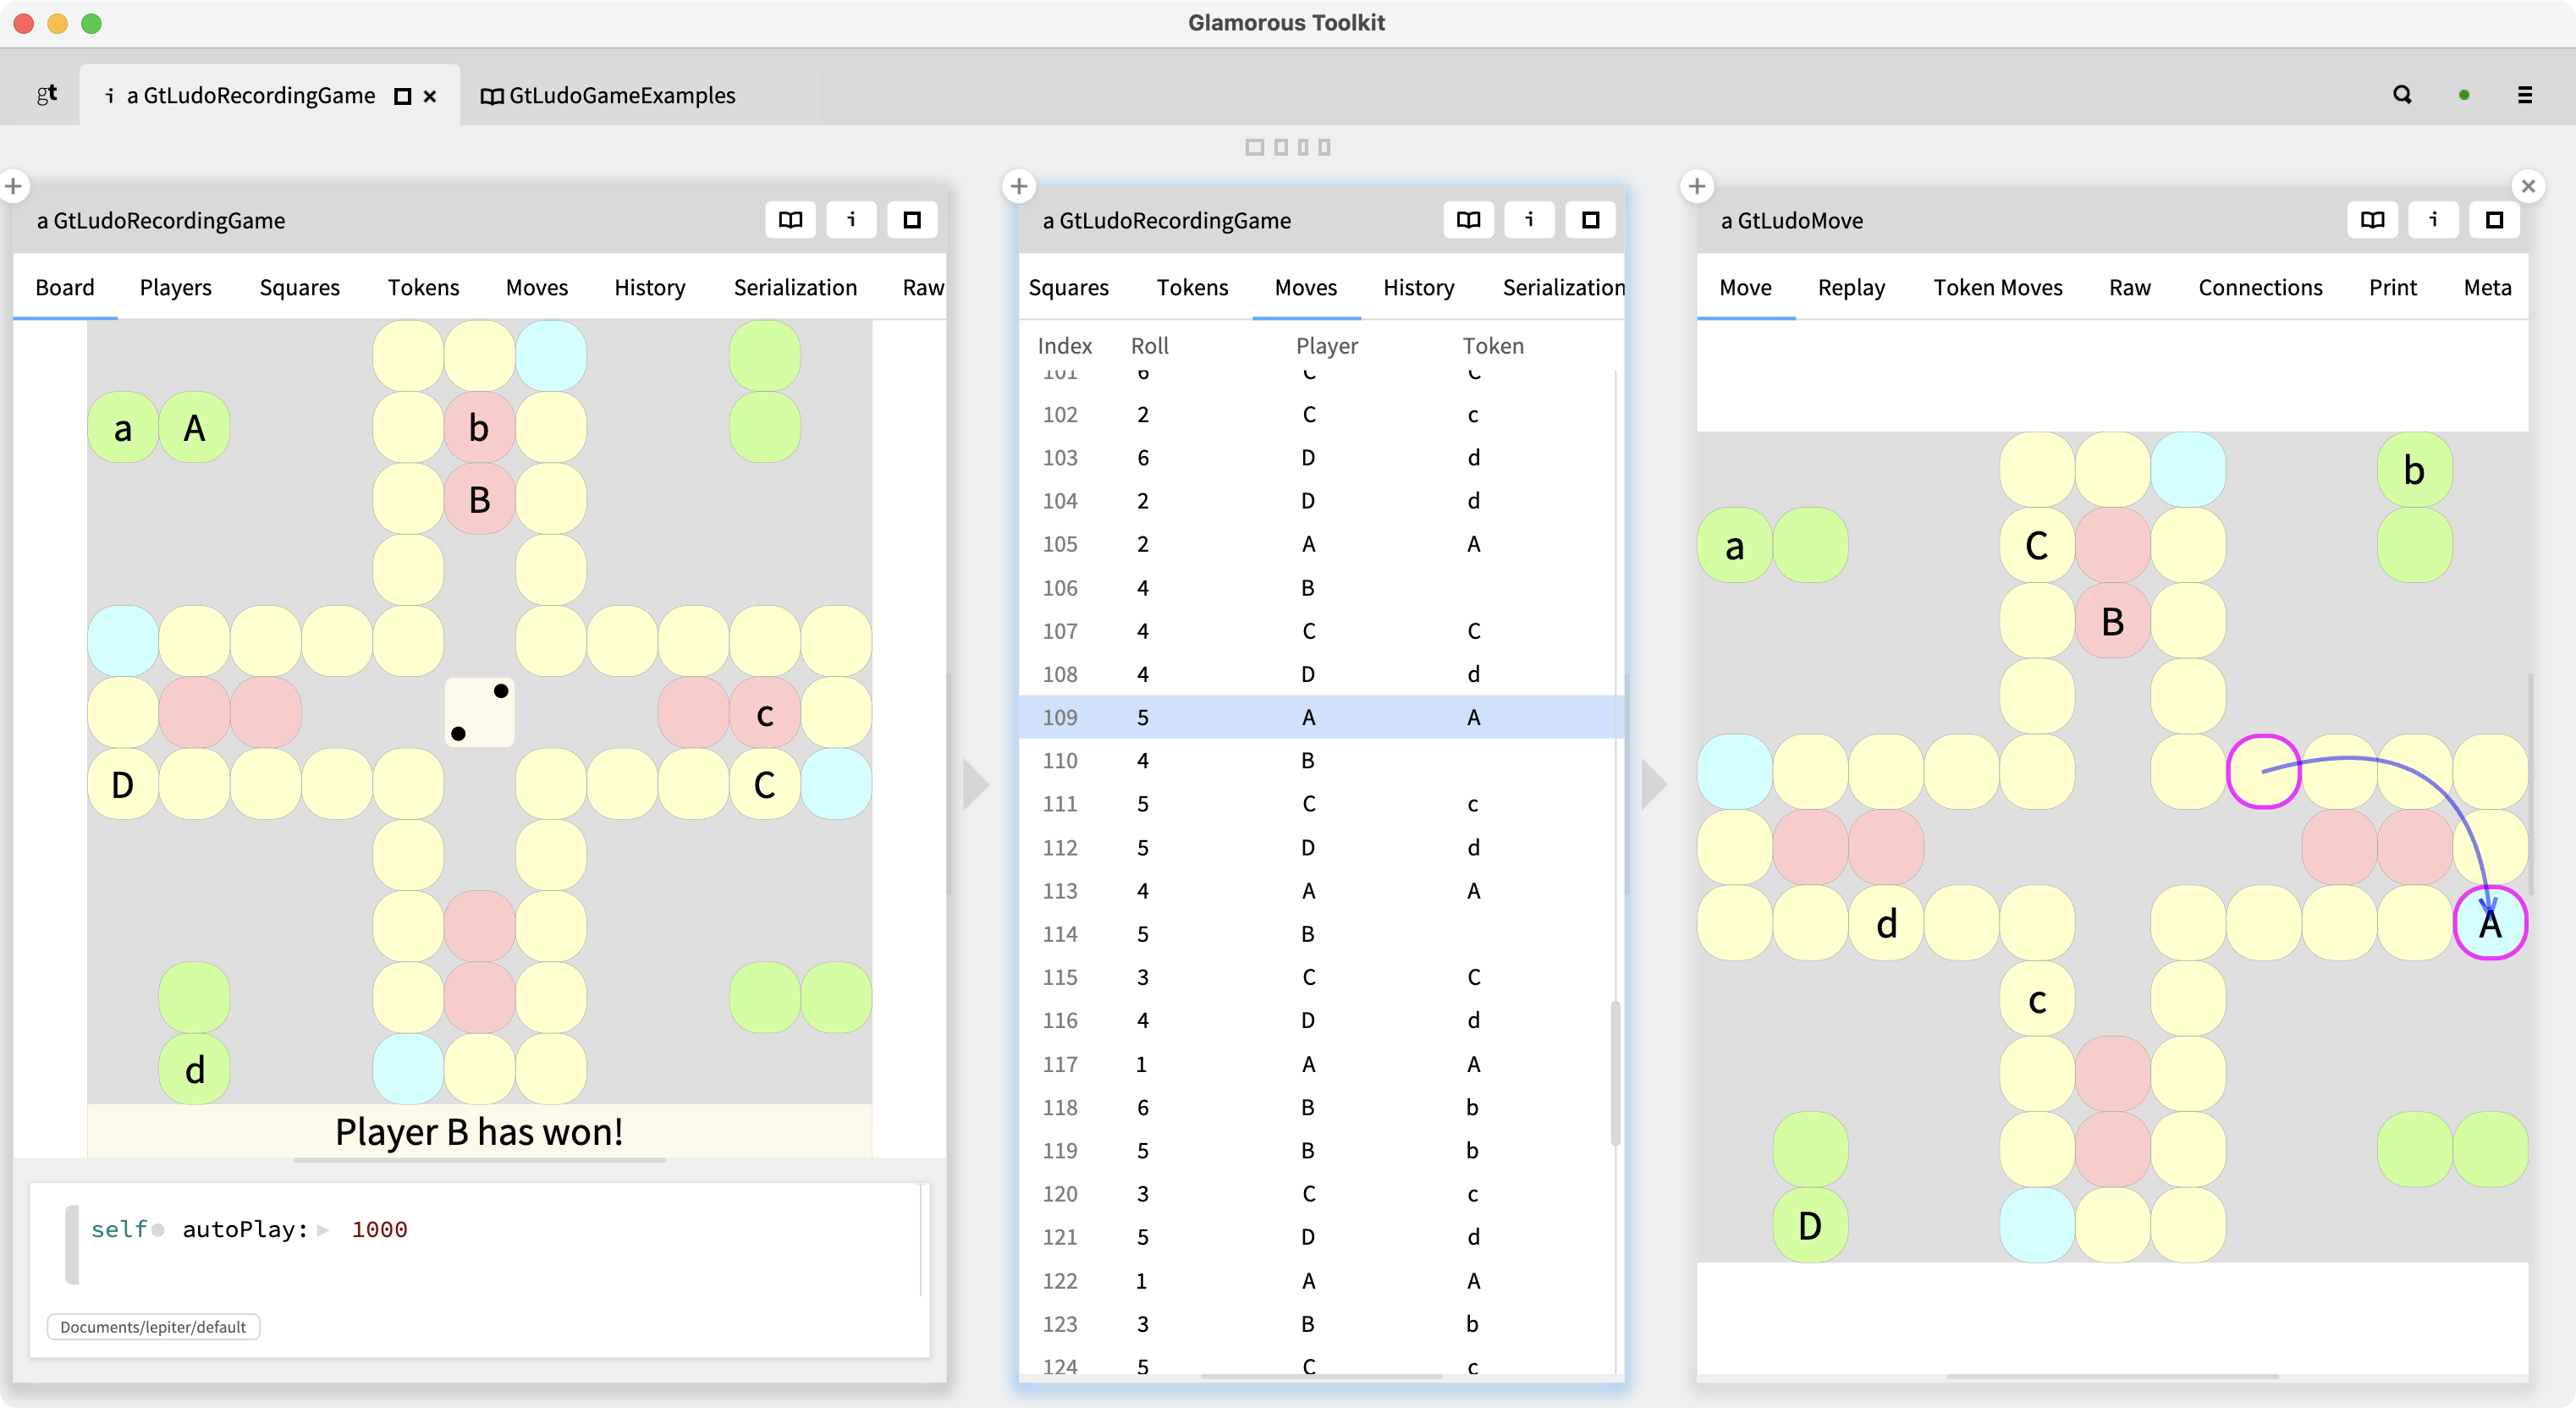
\includegraphics[width=\columnwidth]{customViews}
  \caption{Custom views of a Ludo game.}
  \label{fig:ludoViews}
\end{figure}

As a simple example, consider the Inspector views of a Ludo game implementation in \autoref{fig:ludoViews}.
With a conventional implementation, we can either try to play the game interactively, or we can stare at the source code.
We can also run the tests, but if these are all green, they do not help us to understand the system.
By applying moldable development, we turn questions we have about the game into custom views.

The figure shows three connected custom Inspector views of a running game in the Glamorous Toolkit\footnote{\url{https://gtoolkit.com}} (\GT), a moldable development environment.
In the leftmost pane we see the game GUI as the \st{Board} view.
We can also interact programmatically with the game, evaluating ``\st{self autoPlay: 1000}'' in a contextual playground (a kind of REPL) below the view.
In the second pane we can explore the moves of  the completed game, and in the third pane we can explore individual moves.
The \st{Move} view visualizes the actual move performed in the context of the current game state at that point in time.
Each of these views is achieved with just a few lines of code, and leads to the Ludo game becoming an explainable system that can be explored in ways that are far richer and more intuitive than by trying to read source code.

In a nutshell, Moldable development is a way to make systems explainable by making the domain model of a software system visible and explorable through custom tools.
Of course, this begs the question how to actually apply moldable development in practice.
In our experience applying moldable development to many industrial and open source systems, we have encountered a number of repeating patterns, which we document below.

% ===== Moldable Development Patterns =========================
\section{Moldable Development Patterns}

There are two distinct roles involved in moldable development:
\begin{inparaenum}[(i)]
\item the \emph{Facilitator} is responsible for the technical realization of custom tools, and
\item the \emph{Stakeholder} is responsible for the domain model and questions about the domain that should be answered by the custom tools.
\end{inparaenum}
In a purely technical domain, these two roles can often be played by the same person (\ie a developer), but in general they may be distinct people.

\begin{figure}[h]
  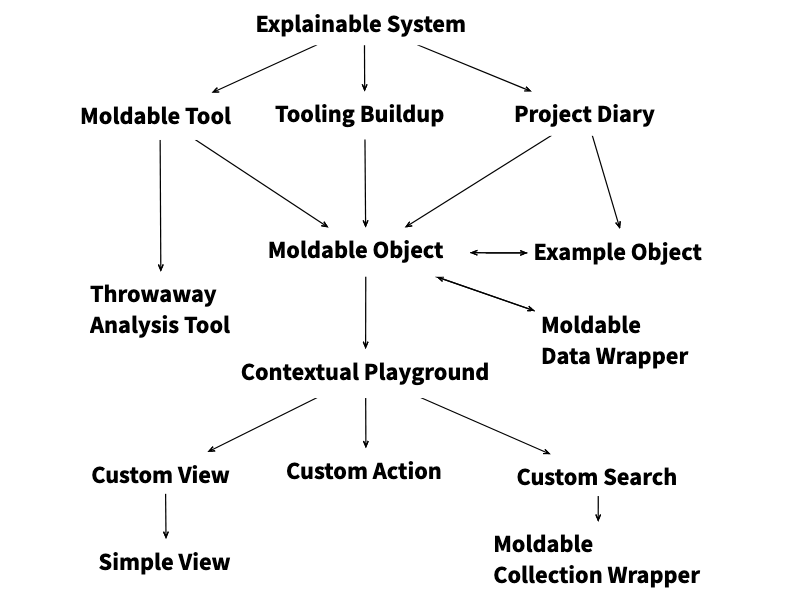
\includegraphics[width=\columnwidth]{map}
  \caption{A map of moldable development patterns.}
  \label{fig:map}
\end{figure}

Moldable development can be understood in terms of a collection of mutually supporting design and process patterns, summarized in \autoref{fig:map}.
These patterns have emerged over several years of experience in developing the Glamorous Toolkit\footnote{\url{https://gtoolkit.com}} moldable development platform, and applying it to numerous systems.
At the root we have the pattern \pattern{explainableSystem}, a software system whose domain model has been exposed with the help of numerous custom tools.
Each custom tool requires the existence of a \pattern{moldableTool}, which can be cheaply adapted with a simple customization.
Some domains require a preliminary phase of \pattern{toolingBuildup}, for example, to create dedicate parsers for programming languages, DSLs or specialized data formats, or bridges to other execution platforms.
A \pattern{projectDiary} is a notebook that serves as a starting point for development tasks.
A \pattern{throwawayAnalysisTool} can be a useful prototype to initially engage a Stakeholder by demonstrating the possibilities of moldable development.

Moldable development itself starts with a \pattern{moldableObject}, a live instance of a domain entity that is explored and molded with custom tools that package the results of exploration tasks.
An interesting instance can be encapsulated as an \pattern{exampleObject}, essentially a unit test that returns a tested object.
An example can be embedded in a project diary notebook page, and can also be used as a moldable object itself for further development tasks.
In case the domain includes already existing data entities, these can be wrapped in a \pattern{viewableDataWrapper} to produce a moldable object.

A moldable object can be explored with the help of its \pattern{contextualPlayground}, a live programming environment bound to the state of a live instance.
Working code can be extracted from such a playground to create custom tools.
The most common of these tools are:
\begin{inparaenum}[(i)]
\item a \pattern{customView}, a dedicated view of an object within a moldable tool such as an object inspector or a code browser, to display or visualize domain-specific information,
\item a \pattern{customAction} that encapsulates a useful domain action, and
\item a \pattern{customSearch}, to perform an ad hoc query over objects reachable from a given moldable object.
\end{inparaenum}
A custom view is frequently a \pattern{simpleView} that can be quickly prototype, and later extended.
A custom search often benefits from a \pattern{collectionWrapper}, to allow the results of a query to be also molded with custom tools.

% ----- Explainable System -------------------------
\subsection*{Explainable System}\label{pat:explainableSystem}

\subsubsection*{Context}
You need to make technical and non-technical decisions about the further development and evolution of a software system, but this is difficult because the system is complex and hard to understand.

\subsubsection*{Problem}
How can you prepare a software system so that various stakeholders (both technical and non-technical) can easily answer questions they have about it?

\subsubsection*{Forces}
Source code is impossible to read at scale.
Static documentation tends to get out of date.
The live, running system is designed to fulfil end user use cases, not answering technical or business questions.
Generic analysis tools and IDEs are unlikely to be able to answer domain-specific questions about your system.
Developing custom tools can be costly and time-consuming.

\subsubsection*{Solution}
Transform the software system into a live domain model in which each domain entity can be interactively explored with the help of custom tools, \ie simple views and visualizations, metrics, queries, and operations.
Leverage open, moldable IDE tools to reduce the cost of building custom tools.
Drive the development of the custom tools by concrete questions you have about the system.

\subsubsection*{Consequences}
The custom tools become part of the live, running system.
Unlike static documentation, the custom tools are more likely to stay in sync with the evolving system.

% ----- Moldable Tool -------------------------
\subsection*{Moldable Tool}\label{pat:moldableTool}

\subsubsection*{Context}
You are developing a complex software system, and find that the existing development tools fall short in supporting domain-specific questions about the software.

\subsubsection*{Problem}
How can you cheaply and effectively extend the development environment with domain-specific tools that address your application domain?

\subsubsection*{Forces}
Generic software tools are fine for answering generic questions, but they do not scale well when addressing domain-specific questions.
(Consider a generic debugger being used to debug an event-driven application\,---\,you want to step through the chain of events, not the stack.)
A plugin-architecture can open up an IDE to new tools, but plugins can be complex and expensive to implement, and they often do not play nicely with existing tools or with each other.

\subsubsection*{Solution}
Make the development tools \emph{moldable} to the \emph{dynamic context} of the artifacts they are intended to work with~\cite{Chis17a}.

A moldable tool makes its core functionality configurable by means of a lightweight mechanism.
For example, a Test Runner in a modern IDE recognizes the presence of test cases by means of various programming conventions, \ie a test case is a method with a standard annotation, or it's a method whose name starts with \st{"test"} and belongs to a class that inherits from a \st{TestCase} class or implements a \st{Test} interface.

By the same token an Inspector can be made moldable by recognizing that an object it is inspecting has one or more custom views defined.
For example, in \autoref{fig:viewCode} we see that inspecting an instance of a \st{GtLudoRecordingGame} yields a custom \st{Moves} view listing the moves played thus far, as the Inspector detects a \st{gtMovesFor:} method defined in the object with a \st{<gtView>} pragma (\ie annotation).
The custom view is defined in a just a few lines of code, creating a \st{columnedList} from the moves.

\begin{figure}[h]
  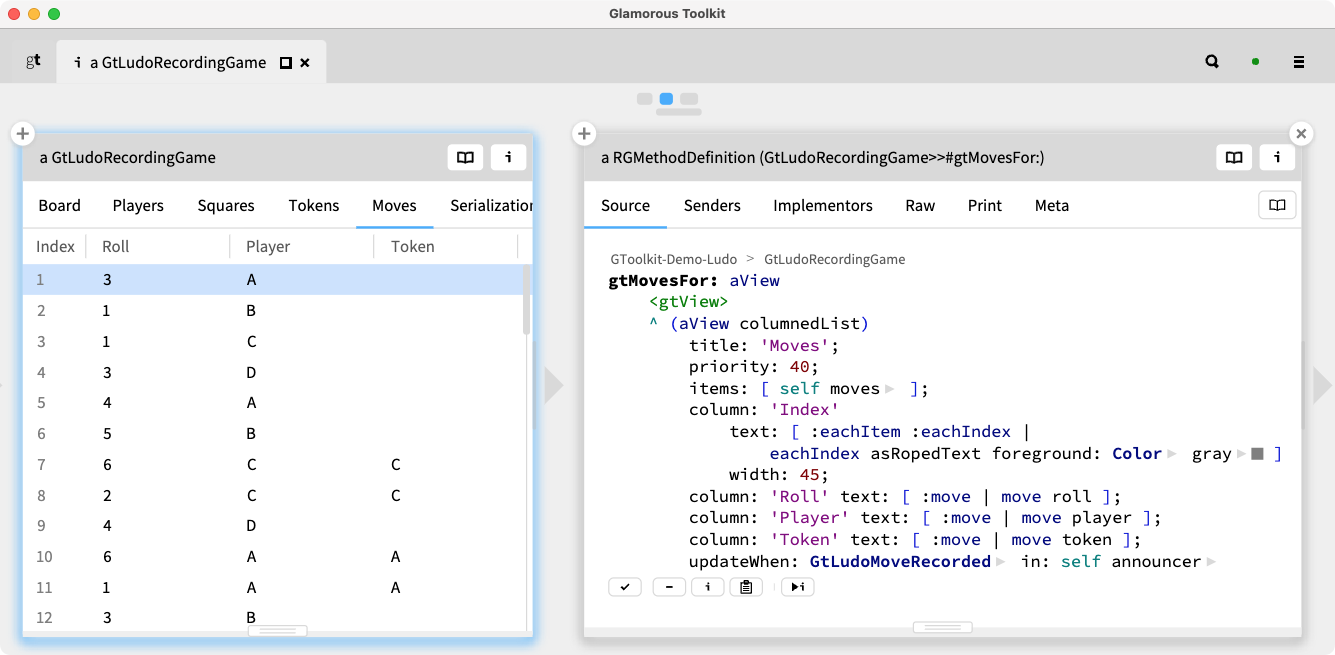
\includegraphics[width=\columnwidth]{viewCode}
  \caption{Defining a custom Inspector view.}
  \label{fig:viewCode}
\end{figure}

The precise mechanism used to mold a tool is not so important, as is the fact that the customizations should be cheap, \ie few lines of code, and \emph{dynamic}, \ie detected at run time.

Other examples include:
\begin{inparaenum}[(i)]
\item a moldable code editor offering alternative views of packages, classes or methods to show dependencies, tests, or other more domain-specific features,
\item a moldable debugger to adapt the stepping behavior for domains such as event-driven applications, or parsing rules,
\item a moldable notebook, supporting domain-specific snippets or annotations.
\end{inparaenum}

\subsubsection*{Consequences}
A moldable tool requires no up-front configuration, since it will be dynamically molded by the artifacts it encounters.
Conversely, since custom tools are an intrinsic part of software systems rather than the IDE, molding happens when needed.

% ----- Tooling Buildup -------------------------
\subsection*{Tooling Buildup}\label{pat:toolingBuildup}
\on{Tooling buildup is the activity you have to perform before you can start the real moldable development. This may have to do with creating parsers for programming languages or data formats of the target domain, bridges to other execution platforms, or any other kind of dedicated tools.}
\on{What makes this a pattern, aside from the fact that it is something you have to do? If it's different each time, then it's not a pattern, is it?}
\subsubsection*{Context}
\subsubsection*{Problem}
\subsubsection*{Forces}
\subsubsection*{Solution}
\subsubsection*{Consequences}

% ----- Throwaway Analysis Tool -------------------------
\subsection*{Throwaway Analysis Tool}\label{pat:throwawayAnalysisTool}
\subsubsection*{Context}
\subsubsection*{Problem}
\subsubsection*{Forces}

\subsubsection*{Solution}
\on{What are the recurring ideas? The purpose is to engage the Stakeholder. Pick some task that will demonstrate the benefit of an explainable system, but without stressing the Stakeholder. The task should be feasible in reasonable time but non-trivial. There should be a clear value for the Stakeholder, that is, do something that the Stakeholder has difficulty with.}

\subsubsection*{Consequences}

% ----- Project Diary -------------------------
\subsection*{Project Diary}\label{pat:projectDiary}
%\on{See \href{https://book.gtoolkit.com/project-diary-dyquv1ad359wsnwasp6hwkgcj}{Project Diary book page}}

\subsubsection*{Context}
You are working on a software project and need to track your progress.

\subsubsection*{Problem}
How can you keep track of decisions, experiments and progress in a moldable development project?

\subsubsection*{Forces}
It's boring to write documentation after the fact, so it is rarely done.
Documentation is not part of the running system, so it distracts you from coding.
Tools for tracking your progress are separate from the code base, so they are commonly out of sync with reality.

\subsubsection*{Solution}
Use a live notebook as the starting point for your project and all of its tasks.
Create a dedicated notebook page for each project, or even each project task, to summarize the goals, and provide pointers to related material.
Use the notebook to keep a diary of your progress.
As the project matures, use the notebook as a draft for the documentation.

For example, in \autoref{fig:projectDiary} we see a live Lepiter page \cite{Girb21a} documenting the task of adding some list views to the Ludo game.

\begin{figure}[h]
  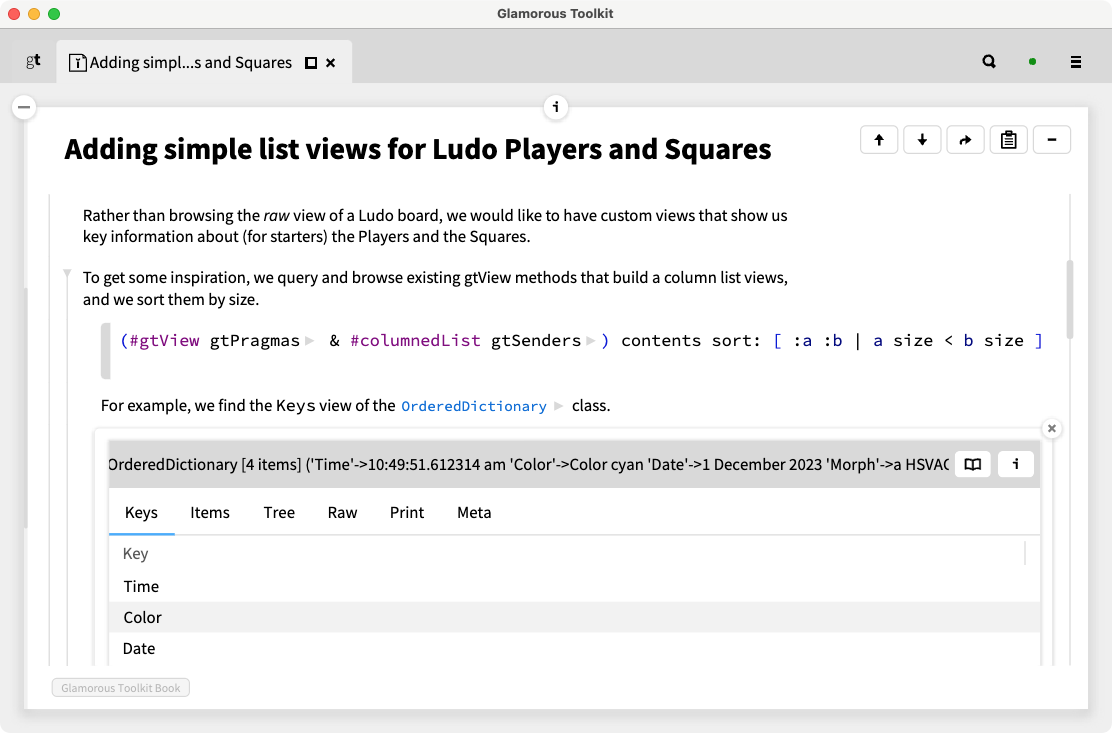
\includegraphics[width=\columnwidth]{projectDiaryExample}
  \caption{Documenting your progress in a live notebook.}
  \label{fig:projectDiary}
\end{figure}

If needed, add code snippets for any setup tasks (e.g., cloning repositories or loading databases).
Also add code snippets to the notebook pages to serve as moldable objects to start coding from.
Extract interesting code snippets as example objects to document interesting use cases, or to serve as tests.

As the project grows, organize the notebook into a main page with an overview, and separate notebook pages for different tasks or groups of related tasks.

Consider using notebook tags to organize your pages implicitly. For example, use a dedicated project tag for all the project pages, and additional tags to indicate their status (``todo'', ``completed'', ``urgent'' \etc).
For example, the ``DRAFT'' tag is used to track pages of the Glamorous Toolkit Book\footnote{The GT Book is the documentation of the Glamorous Toolkit Moldable Development Environment implemented as a live notebook. A static snapshot is also available: \url{https://book.gtoolkit.com}.} that require further editing.

At the end of a project, consider recycling and rewriting the project pages to create documentation. In this way the diary can serve as a rough draft.

\subsubsection*{Consequences}

A live notebook is an integral part of the project, and evolves together with other software artifacts.
Notebook pages can express tasks in various stages of completion, so can be used as starting points for further development tasks.
Notebooks can serve not only to track progress, but also as documentation for both technical and non-technical stakeholders.

% ----- Moldable Object -------------------------
\subsection*{Moldable Object}\label{pat:moldableObject}
%\on{See \href{https://book.gtoolkit.com/moldable-object-9jkob03k21sbjujct0kh60016}{Moldable Object}}
\subsubsection*{Context}
You have your basic infrastructure in place, and want to start the process of creating an explainable system, either from scratch, or based on some existing software or data.

\subsubsection*{Problem}
Where do you start coding an explainable system?

\subsubsection*{Forces}
As a programmer, you want to quickly get feedback about the code you are writing.
When you write code in a classical IDE code editor, you are several steps away from seeing the consequences of your coding.
To write unit tests, you must already have an idea what behavior you want to test and what the results should be.

\subsubsection*{Solution}
Start coding by inspecting a moldable object, that is, a live instance of the class you are coding, not in a code editor.
Then incrementally pose domain-specific questions, find the answers by exploring and interacting with the object, and then turn those answers into custom tools, behaviors and tests.

Moldable development is about making systems explainable with the help of custom tools, which means that you need to start the process by asking questions that you want to answer.
In most cases you can't immediately start building the custom tools, but rather you need to explore the domain objects to understand how to answer the question.
Once you know how to get the answer, you can turn the exploration steps into a custom tool.
Starting with a live object means that you can immediately start the exploration process.
Turning the exploration of an object into a custom tool is the process of molding it, hence we call it a ``moldable object.''

How do you obtain a moldable object?
\begin{itemize}[---]
\item \emph{You already have a class:} create a \pattern{projectDiary} notebook page containing a code snippet to create an instance of the class, and start from there.
\item \emph{You don't have a class:} start instead with a code snippet that instantiates an empty class, and then prototype the behavior.
\item \emph{You have a test case:} turn the test case into an \pattern{exampleObject} and start from there.
\item \emph{You have some data:} wrap the data as a \pattern{viewableDataWrapper}.
\end{itemize}

In \autoref{fig:stackMachine} we see an initial notebook page in which we start to explore an instance of a new \st{StackMachine} class that we create with a \emph{fixit} action:
The wrench icon indicates that the class does not exist, so before we can evaluate the expression and inspect the new, moldable object, we must select one of the suggested fixes, in this case, to create a new class.

\begin{figure}[h]
  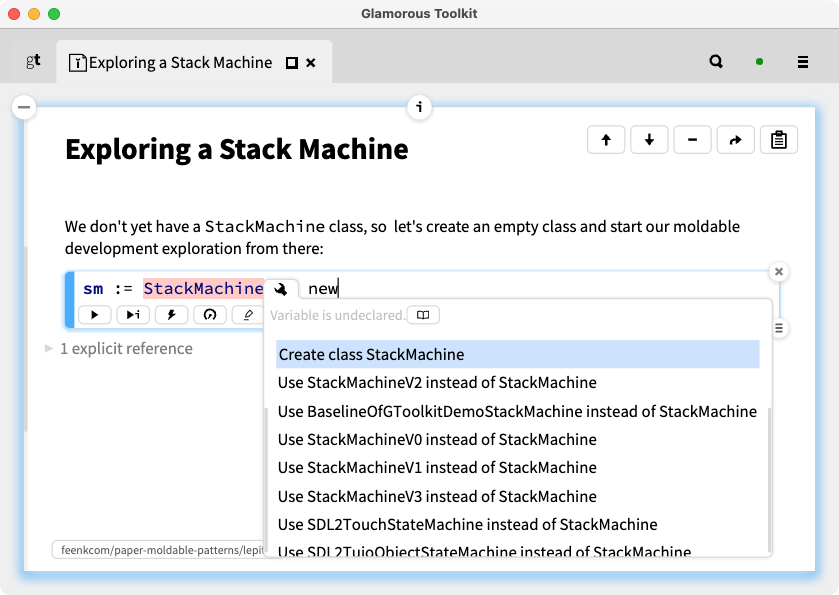
\includegraphics[width=\columnwidth]{stackMachine}
  \caption{Creating a fresh, moldable object for a new class.}
  \label{fig:stackMachine}
\end{figure}

Once we have created the missing class and start to inspect it, we can start to ask questions, such as \emph{What is the number of items in the stack?}, \emph{What is the state of the stack?}, and \emph{How can we push new items onto the stack?}
We can use a \pattern{contextualPlayground} to write experimental code, that we later extract as methods, and as we answer questions we can create small custom tools, such as a \pattern{customView} or a \pattern{customAction}.

Whenever we identify an interesting state of our moldable object, we can extract it as an \pattern{exampleObject} that we can use as a test case, or as a starting point for further moldable development.

\subsubsection*{Consequences}
Instead of writing code in a text editor in the context of the source code of a class, you are always working in the context of a live object, whose behavior can be immediately explored.

Instead of writing hypothetical code that you must afterward test, you start by prototyping code and then extracting new behavior.

Instead of trying to program custom tools in a vacuum, you first explore and prototype answers to questions, and then extract the code you need to create a custom tool.

% ----- Example Object -------------------------
\subsection*{Example Object}\label{pat:exampleObject}

% --- CONTINUE HERE
\here

\on{See \href{https://book.gtoolkit.com/example-object-dyquv1b6xptl2c0ayhgb376bw}{Example Object book page}}

\subsubsection*{Context}
\subsubsection*{Problem}

How do you organize examples for testing and documentation?

\subsubsection*{Forces}

Concrete examples are need for many purposes, such as documentation, testing, and exploration.
Examples can be complex to set up.Unit tests consume examples, but they are only accessible if a test fails.

\subsubsection*{Solution}

Wrap examples as (instance) methods that optionally evaluate some tests (assertions), and return the example instance. Each example may also use one or more examples as the initial setup for the new example.

To start, you need a modified unit testing framework in which tests return the exercised fixture, namely, an example. In GT, you create an Example by defining a parameterless method that has a \st{gtExample} pragma, and returns an object. (A similar framework for Java is JExample.)

Here's a simple example that returns a parse node for the parsed string '3+4', and asserts that the result is not fully reduced (evaluated).

%a3plus4
%	<gtExample>
%	| result |
%	result := self parseExpression: '3+4'.
%	self assert: result isReduced not.
%	^ result
    
Unlike normal test methods, examples can be composed. For example, this example method performs an evaluation step on the previous example, and returns the fully reduced expression node, asserting that no more evaluation steps can be performed.

%a3plus4is7
%	<gtExample>
%	| result context |
%	context := self a3plus4 asContext.
%	result := context step.
%	self assert: result isSPLValue.
%	self assert: result value equals: 7.
%	^ result
    

\subsubsection*{Consequences}

Examples can be run just like classical unit tests.

When an example fails, its dependent examples do not need to be run.

When an example succeeds, it can be inspected, used as a moldable object to start coding, or embedded as a live example snippet within a notebook page to illustrate some point. (The example snippets above illustrate this.)

When you are searching for usages of an API, not only do you find examples that illustrate the usage, but by running the example you obtain a live instance that you can explore.

% ----- Viewable Data Wrapper -------------------------
\subsection*{Viewable Data Wrapper}\label{pat:viewableDataWrapper}
\on{See \href{https://book.gtoolkit.com/viewable-data-wrapper-9jkob08ts9ihwg72kvyccl5ff}{Viewable data wrapper book page}}
\subsubsection*{Context}
\subsubsection*{Problem}

When you explore data with a platform such as GT, the views you obtain reflect the low-level data structures used to represent the data, not the underlying domain concepts. How can we add appropriate high-level views to the data?

\subsubsection*{Forces}

When we explore data, we represent them using suitable low-level data structures.

Data structures (lists, dictionaries) reflect the representation of data, not their interpretation.

To analyze and explore data, we need higher-level views that reflect our understanding of the data.

\subsubsection*{Solution}

Wrap each kind of data in a dedicated class reflecting the problem domain. 

As you explore the data, introduce custom views to the domain class that reflect answers to questions you ask about the data.

Extract the data of interest. This might be data sitting in your file system (for example, a CSV file), or data retrieved from a website.

A classical example can be seen in Working with a REST API: the GitHub case study .

We obtain a Dictionary representation of JSON data about the feenk GitHub organization:

url := 'https://api.github.com/orgs/feenkcom'.
json := ZnClient new get: url.
dictionary := STON fromString: json.
  
If we explore this object, we just see the keys and values of the raw downloaded data. From this view, of course we can explore the data by navigating the Dictionary views, or by programatically exploring other paths using the Inspector Playground, but we cannot add or tailor views to specifically support the GitHub Organization domain.

We address these problems by wrapping the raw data as a dedicated GhOrganization object, as follows:

GhOrganization new rawData: dictionary.
  
Now we can add custom views specific to this domain, for example, listing the Repositories of an organization, or the most recent GitHub events. For each new domain concept, we introduce a dedicated wrapper object, so we can navigate the entire model via the domain concepts.

\subsubsection*{Consequences}

% ----- Contextual Playground -------------------------
\subsection*{Contextual Playground}\label{pat:contextualPlayground}
\on{See \href{https://book.gtoolkit.com/contextual-playground-9jkob08mw269cpxowmbe0ld8i}{Contextual Playground book page}}
\subsubsection*{Context}
\subsubsection*{Problem}

When we code new behavior as methods, we must must repeatedly change our context to incrementally develop the logic. Testing the code requires a separate setup. How can we efficiently prototype and test the new behavior?

\subsubsection*{Forces}

An editor for coding new methods typically provides no facilities for testing the code.

Setting up code to prototype and test logic can be cumbersome.

Writing tests first for parts of the logic of a complex method may can be overkill.

\subsubsection*{Solution}

Prototype new behavior in the Playground of a Moldable object, i.e., an Inspector on a live instance of the class. The Playground will be bound to the context of the instance, so self and all slots can be accessed exactly as they would in a running method.

From the moldable object you can navigate to any parts of the instance, to explore the APIs, or to test experimental code.

Code snippets that work as expected can then be copy-pasted to existing methods, or extracted to new methods using an Extract method refactoring.

\on{See the Steps in the book page}

\subsubsection*{Consequences}

% ----- Custom View -------------------------
\subsection*{Custom View}\label{pat:customView}
\on{See \href{https://book.gtoolkit.com/viewable-entity-9jkob0898tctthh5o3m23fv4e}{Viewable entity book page}}
% AKA Viewable Entity
\subsubsection*{Context}
\subsubsection*{Problem}

As you explore a live model, you may find yourself repeatedly navigating through multiple inspector views to reach the information you want. How can you make this process more efficient?

\subsubsection*{Forces}

Navigating to the data you want to reach may entail a sequence of operations, either clicking in views, or evaluating Playground snippets, to reach a new Inspector instance.

The sequence of steps may be cumbersome to follow repeatedly.

\subsubsection*{Solution}

Turn interesting data into a viewable entity . Extract the navigation steps into a new custom view for the moldable object you start navigating from. Possibly start with a simple forward view to an existing view of the target data, and later refine this into a dedicated view.

\on{See the Steps in the book page}

\subsubsection*{Consequences}

% ----- Simple View -------------------------
\subsection*{Simple View}\label{pat:simpleView}
\on{See \href{https://book.gtoolkit.com/simple-view-dyquv19x8xwi85g99n0akc5lu}{Simple view book page}}
\subsubsection*{Context}
\subsubsection*{Problem}

How much effort should you invest into creating a new view?

\subsubsection*{Forces}

There are many different kinds of views; how can you tell which one is most suitable?

\subsubsection*{Solution}

A view exists only to answer a question about a domain object. Pick the simplest view that will answer the question. Only refine the view if it can answer more questions.

\on{See the Steps in the Book page.}

\subsubsection*{Consequences}

% ----- Custom Action -------------------------
\subsection*{Custom Action}\label{pat:customAction}
\on{See \href{https://book.gtoolkit.com/custom-action-7ed0nuwfqc5qp8b1b257cavgy}{Custom Action book page}}
\subsubsection*{Context}
\subsubsection*{Problem}

As you are developing an explorable model of your application, you may find yourself repeatedly evaluating the same code snippets to perform a given action. How can you streamline these tasks?

\subsubsection*{Forces}

Repeated tasks are annoying and time-consuming.

Remembering how to perform common tasks increases cognitive overload.

\subsubsection*{Solution}

Add a custom action button to the key objects involved in the repeated tasks, encapsulating the boilerplate code to perfom them.

\on{See the Steps in the Book page.}

\subsubsection*{Consequences}

% ----- Custom Search -------------------------
\subsection*{Custom Search}\label{pat:customSearch}
\on{NB: New pattern}
\subsubsection*{Context}
\subsubsection*{Problem}
\subsubsection*{Forces}
\subsubsection*{Solution}
\subsubsection*{Consequences}

% ----- Collection Wrapper -------------------------
\subsection*{Collection Wrapper}\label{pat:collectionWrapper}
\on{See \href{https://book.gtoolkit.com/collection-wrapper-dyquv1bb9krkve76ncq4kyxr7}{Collection wrapper book page}}
\subsubsection*{Context}
\subsubsection*{Problem}

What is the best way to provide custom views of collections of domain objects, when they may occur in many different contexts?

Example:
When we explore a website, we have lists of links in a website or a webpage, we have lists of internal links, external links, broken links, or queries returning links that match some text. Providing custom views for each of these is tedious and leads to much duplicated code.

\subsubsection*{Forces}

It is common to have to deal with collections of domain objects, but it is tedious to create custom views for each of these. Collections may form part of the internal state of a domain object, such as a website containing pages, or a page containing links, but a collection may also be returned by a query, such as a Spotter search, for example the set of web pages containing a certain string in their title or page contents.

Raw collections have uninteresting views. Collections are very similar and have a lot of boilerplate code. Many views are essentially collections, and have similar implementations.

\subsubsection*{Solution}

Wrap collections of domain objects in a dedicated group wrapper, and give it dedicated views, actions and searches.

Create a dedicated wrapper for a collection of domain entities. An example is WebPageGroup , which wraps a collection web pages.

Have the collection wrapper use the TGtGroupWithItems trait. This trait has an items slot for the wrapped collection, and provides a large number of Collection methods to make the trait user behave like a Collection.

In case there are other classes that share views, actions and searches with the collection wrapper, consider putting these in a shared trait as well. For example, a website is also a collection of pages. We put the shared views and other behaviour in the trait TWebPageGroup . The trait users are AWebsite and WebPageGroup.

Wherever you need to show a collection of these objects, just forward the view to the wrapper to avoid duplicating the view code. 
% See TWebPageGroup>>#gtReachablePagesFor: .

% If you have gtSearches, be sure they return the collection wrapper and not the raw collection, using the sendCategory: message, for example, TWebPageGroup>>#gtSpotterForPageContents: .

\subsubsection*{Consequences}

%% The next two lines define the bibliography style to be used, and
%% the bibliography file.
\bibliographystyle{ACM-Reference-Format}
\bibliography{moldablePatterns}

\end{document}
\endinput

% ===== TEMPLATES =========================

% ----- PATTERN -------------------------
\subsection*{PATTERN}\label{pat:PATTERN}
\subsubsection*{Context}
\subsubsection*{Problem}
\subsubsection*{Forces}
\subsubsection*{Solution}
\subsubsection*{Consequences}

\begin{inparaenum}[(i)]
\item
\item
\end{inparaenum}

